\documentclass[addpoints,12pt]{exam}
%\documentclass[12pt]{article}
\usepackage[letterpaper, margin=0.75in]{geometry}
\usepackage{graphicx}
\usepackage{enumitem}
\usepackage{booktabs}
\usepackage{tabularx}
\usepackage{color}

\begin{document}
\footer{}{Page \thepage\ of \numpages}{}

\begin{center}

\includegraphics[width=10cm]{../images/logo.png}
\end{center}

\begin{center}
\noindent{\LARGE Conceptual Physics \\ Homework Packet 4\\ Solutions\\}
\end{center}
 
\clearpage

\begin{flushright}
Score: \hspace{0.2in} / \numpoints ~ points
\end{flushright}

\begin{questions}
	
\question[6]
\begin{parts}
	\part What is the difference between an \textit{elementary} and a \textit{composite} particle?
		\begin{TheSolution}
			A composite particle can be broken into smaller particles, whereas an elementary particle cannot.
		\end{TheSolution}
	\part List 2 \textit{elementary particles}:
		\begin{TheSolution}
			There are 17 known fundamental particles. These include:
			\begin{itemize}
				\item Quarks (up, down, charm, etc.)
				\item Leptons (electron, muon, tao, neutrinos, etc.)
				\item Photons (light of any frequency)
				\item Bosons (W and Z bosons, gluon, Higgs)
			\end{itemize}
		\end{TheSolution}
	\part List 2 \textit{composite particles}:
		\begin{TheSolution}
			The main ones we covered in class are:
				\begin{itemize}
					\item Protons (composed of quarks)
					\item Neutrons (also composed of quarks)
				\end{itemize}
		\end{TheSolution}
\end{parts}

\question[6] Plutonium-240 ($Pu^{240}$) decays by emitting a helium-4 nucleus.
	\begin{parts}
		\part How many protons are in plutonium-240?
			\begin{TheSolution}
				\textbf{94.} From the periodic table, we see that the atomic number of plutonium is 94.
			\end{TheSolution}
		\part How many neutrons are in plutonium-240?
			\begin{TheSolution}
				\textbf{146.} We know that the nucleus has 240 neutrons +  protons, and that it has 94 protons. It therefore has 240-94=146 neutrons.
			\end{TheSolution}
		\part When a plutonium-240 nucleus decays and emits a helium-4 nucleus, what element does it turn into? How many protons and neutrons are in this nucleus?
			\begin{TheSolution}
				Plutonium-240 looses 2 protons, so it's atomic number goes from 94 to 92: this is uranium on the periodic table. It also lost 2 neutrons, so the uranium nucleus has 146-2 = 144 neutrons in it. This is uranium-236
			\end{TheSolution}
	\end{parts}
	
	\question[4] Primordial light from the big bang continues to exist in our universe, but it has been highly \textit{red-shifted} due to the universe's expansion, to the point that it is in the microwave region. This is known as the \textit{cosmic microwave background} (CMB) and physicists are highly interested in measuring it because we can use it as a probe of the early universe.
	\begin{parts}
		\part In the past, was the \textit{frequency} of the CMB greater, smaller or the same as it is now?
			\begin{TheSolution}
				\textbf{Greater.} When light is redshifted, its frequency goes down - therefore in the past the frequency had to be greater than it is now.
			\end{TheSolution}
		\part In the past, was the \textit{wavelength} of the CMB greater, smaller or the same as it is now?
			\begin{TheSolution}
				\textbf{Smaller.} When light is redshifted, its wavelength increases - therefore in the past the wavelength had to be smaller than it is now.
			\end{TheSolution}
	\end{parts}
	
	\clearpage
	\question[10] There is a gravitational field surrounding the Earth and Moon.
	\begin{parts}
		\part Using field lines, draws the gravitational field around the Earth and Moon.
			\begin{center}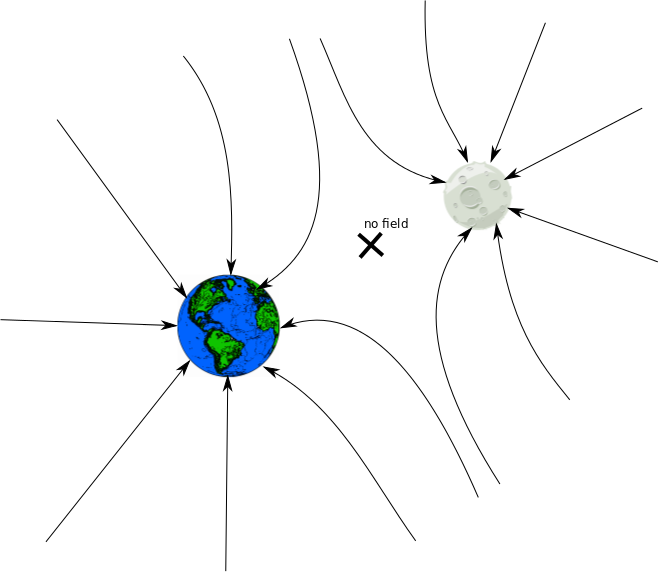
\includegraphics[width=3.5in]{../images/earthMoon_sol.png}\end{center}
			
		\part Using a ``field of arrows", draw the gravitational field around the Earth and Moon.
			\begin{center}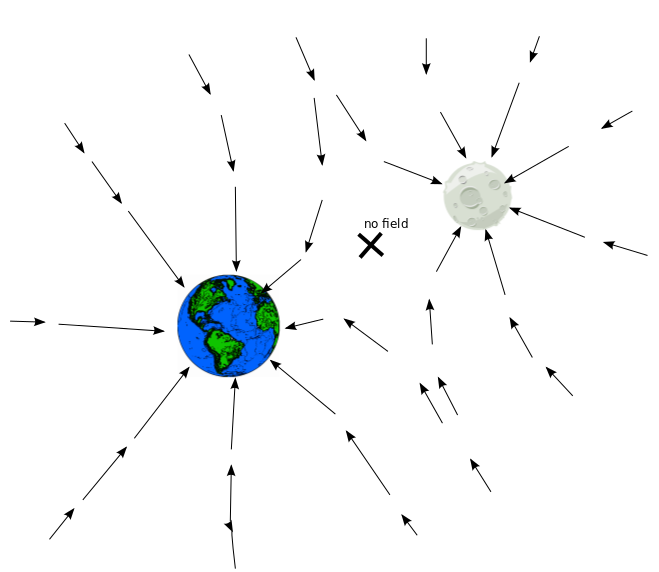
\includegraphics[width=3.5in]{../images/earthMoon_sol2.png}\end{center}
			
		\part There is a point at which the gravitational field is zero. Indicate this point on each of the above diagrams for part (a) and (b).
		\part What force would a test mass experience at the location where the gravitational field is zero?
			\begin{TheSolution}
				It would experience no force.
			\end{TheSolution}
	\end{parts}
	
	\clearpage
	\question[6] When you stand on the surface of the Earth, you experience the full strength of its gravitational field.
	\begin{parts}
		\part What happens to the strength of this gravitational field, if you were to dig deep into the Earth? (Does it increase, decrease, or stay the same?) Please explain your reasoning. Hint: Think about what is generating the gravitational field, and think about the pull of the earth beneath and \textit{above} you as you did deeper.
			\begin{TheSolution}
				\textbf{Decrease.} As you dig under ground, the earth above you pulls you ``up" while the rest of the earth would pull you ``down". The two forces are acting against each other, and so the net force you feel from gravity decreases. Since the field is directly proportional to the force, this means that the field decreases.
			\end{TheSolution}
		\part What is the strength of the Earth's gravitational field, at the center of the Earth?
			\begin{TheSolution}
				\textbf{Zero.} At the center of the earth, you have an equal amount of earth on all sides of you. Therefore, you are being pulled equally in all directions: The forces would all cancel, and you would feel zero force. Therefore, the field at the center must be zero.
			\end{TheSolution}
		\part From this reasoning, draw the gravitational field (as arrows or lines, whichever you prefer) for a hollow sphere using the cross-section provided bellow.
			\begin{TheSolution}
			\begin{center}
			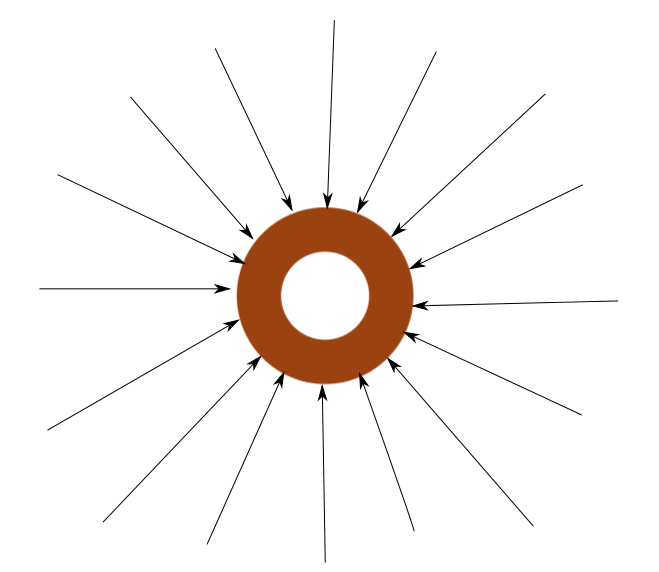
\includegraphics[width=4in]{../images/hollow_sol.png}
			\end{center}
			There is no field in the center.
			\end{TheSolution}
	\end{parts}
	
\end{questions}








\end{document}